\documentclass[spanish]{beamer}
\usepackage[ansinew]{inputenc} % Acepta caracteres en castellano
\usepackage[spanish]{babel}    % silabea palabras castellanas
\usepackage{amsmath}
\usepackage{amsfonts}
\usepackage{amssymb}
\usepackage{dsfont}
\usepackage{graphicx}
\usepackage{geometry}
\usetheme{Madrid}
\usecolortheme{beaver}
\usepackage{textpos}
% Logo  en el comienzo 
\addtobeamertemplate{frametitle}{}{%
\begin{textblock*}{100mm}(.85\textwidth,-1cm)
{\includegraphics[height=0.4in, keepaspectratio=true]{/Users/luisnunez/Dropbox/MisDocumentos/UIS/UISImagenInstitucional/UISLOGO.png}}
\end{textblock*}}

\begin{document}

\title{\textbf{Principios Variacionales} }
\author[L.A. N��ez]{\textbf{Luis A. N��ez}}  
\institute[UIS]{\textit{Escuela de F�sica, Facultad de Ciencias, } \\
\textit{Universidad Industrial de Santander, Santander, Colombia } \\
{\includegraphics[height=0.4in, keepaspectratio=true]{/Users/luisnunez/Dropbox/MisDocumentos/UIS/UISImagenInstitucional/UISLOGO.png}}
}
\date{\today}
\maketitle


\begin{frame}
\frametitle{Agenda}
  \tableofcontents
\end{frame}


%%%%% Diapo 1
  \section{Extremos de un funcional}
\frame{
  \frametitle{Extremos de un funcional}
   \begin{itemize}  
  	\item<1-> En los problemas de extremos del c�lculo diferencial se busca el valor de una variable $x$ para el cual una funci�n $g = g(x)$ es m�xima o m�nima. 
  	\item<2-> En los problemas de extremos en el c�lculo variacional se busca una funci�n $y(x)$ con cual un funcional, $I=\mathcal{F}[y(x)]$, sea extremo (m�ximo o m�nimo). 
	\item<3-> Entonces anularemos las variaciones del funcional, $\delta I = \delta \mathcal{F}[y(x)] = 0$, para determinar la $y(x)$ que lo hace extremo.
			\begin{figure}[t]
			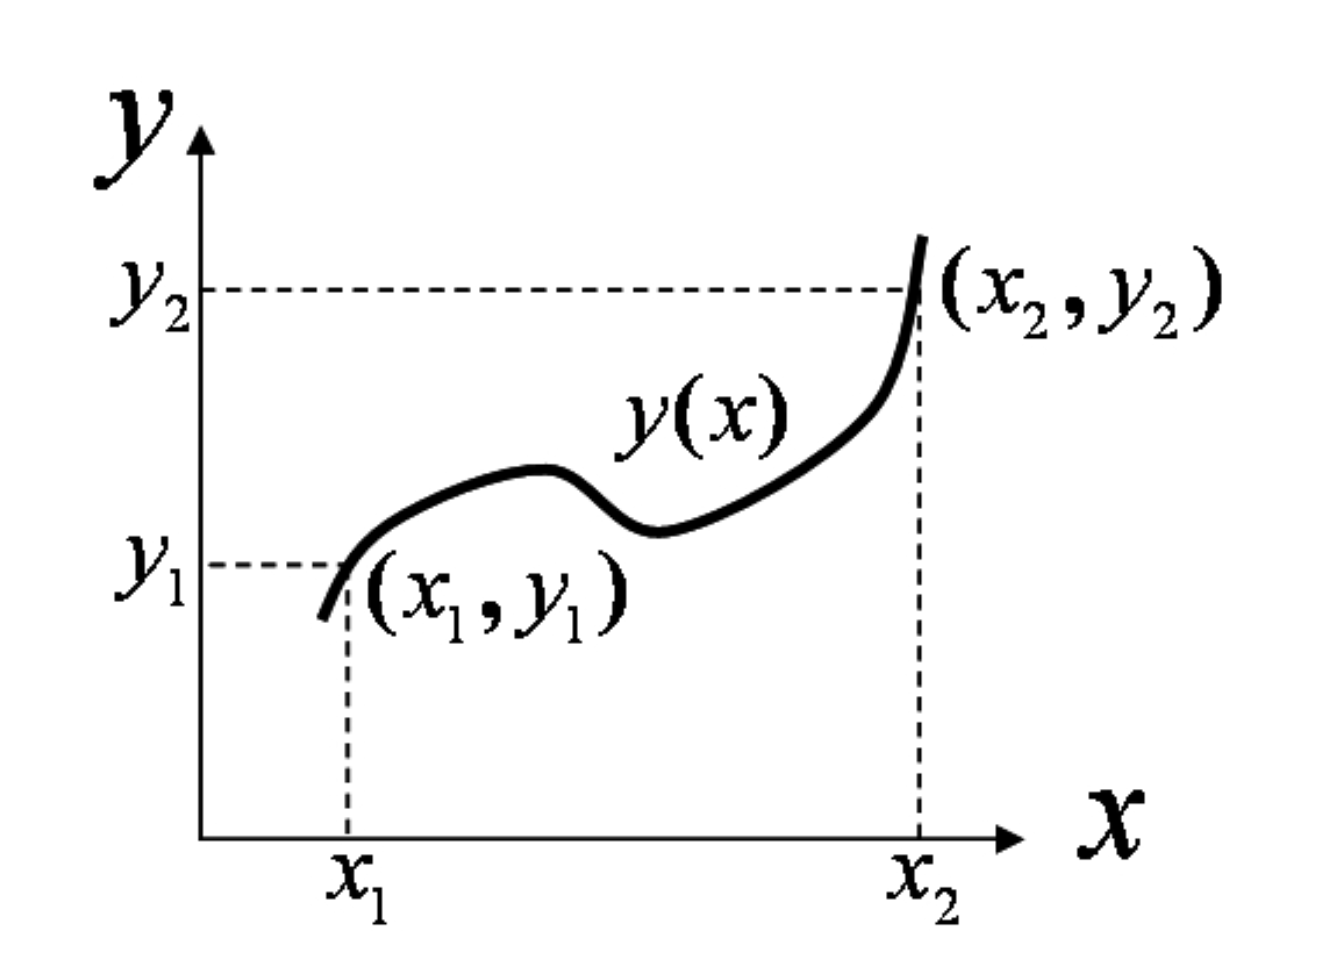
\includegraphics[width=1.4in]{Figuras/Trayectoria.png} \hspace{1cm} 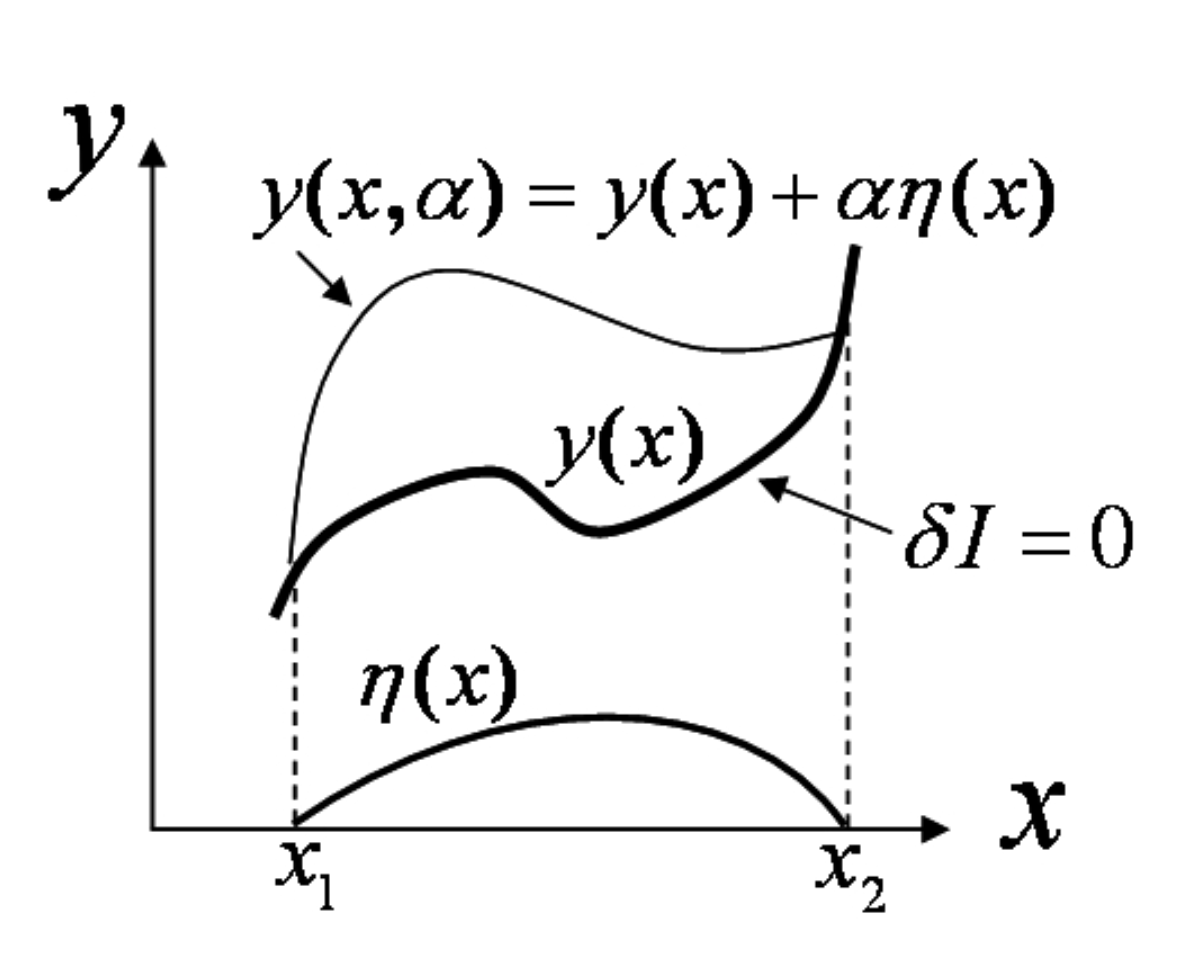
\includegraphics[width=1.4in]{Figuras/TrayectoriaPerturbada.png} 
   		         \end{figure}
    \end{itemize}
}
%%%%% Diapo 2
\section{Trayectorias cercanas a la extrema}
\frame{
  \frametitle{Trayectorias cercanas a la extrema}
  \begin{itemize}  
  	\item<1->  Sea $y(x)$ la funci�n que hace extremo el funcional $I = \mathcal{F}[y(x)] = \int_{x_1}^{x_2} {\rm d}x \; f(y(x), y^{\prime}(x), x)$. 
	\item<2->  Consideremos todas las funciones cercanas a $y(x)$ de la forma $y(x,\alpha) = y(x) + \alpha \eta(x)$, con lo cual $y(x, 0) = y(x)$
	\item<3->  La funci�n $\eta(x)$ es diferenciable y $\eta(x_1) = \eta(x_2) = 0$, con lo cual $y(x_1, 0) = y(x_1) \equiv y_1$ y consecuentemente $y(x_2, 0) = y(x_2) \equiv y_2$
	\item<4->  Entonces hemos transformado el funcional en una funci�n $I(\alpha) = \mathcal{F}[f(x, \alpha)] = \int_{x_1}^{x_2} {\rm d}x \; f(y(x, \alpha), y^{\prime}(x, \alpha), x)$
	\item<5-> Sabemos como buscar los extremos de una funci�n $\left.\frac{{\rm d} I(\alpha)}{{\rm d} \alpha}\right|_{\alpha=0} = 0$
	\item<6-> Al evaluar $\alpha = 0$ garantizamos que obtenemos la $y(x)$ que hace extremo el funcional $I$.  
  \end{itemize}
}

%%%%% Diapo 3
\section{Variaciones de un funcional}
\frame{
  \frametitle{Variaciones de un funcional}
  \begin{itemize}  
  	\item<1-> La derivada $\frac{{\rm d} I(\alpha)}{{\rm d} \alpha} = \int_{x_1}^{x_2} \frac{{\rm d} f\left(y(x, \alpha), y^{\prime}(x, \alpha), x\right)}{{\rm d} \alpha} {\rm d} x$
	\item<2-> Equivalentemente $\frac{{\rm d} I(\alpha)}{{\rm d} \alpha} = \int_{x_1}^{x_2}\left[\frac{\partial f}{\partial y} \frac{\partial y(x, \alpha)}{\partial \alpha}+\frac{\partial f}{\partial y^{\prime}} \frac{\partial y^{\prime} (x, \alpha)}{\partial \alpha} \right] {\rm d} x $
	\item<3-> Donde $\frac{\partial y(x, \alpha)}{\partial \alpha}  =\eta(x)$ y adem�s $\frac{\partial y^{\prime}(x, \alpha)}{\partial \alpha}  =\frac{\partial}{\partial \alpha}\left(\frac{{\rm d} y}{{\rm d} x}\right)=\frac{{\rm d}}{{\rm d} x}\left(\frac{\partial y}{\partial \alpha}\right)=\frac{{\rm d} \eta}{{\rm d} x}$
	\item<4-> Con lo cual $\frac{{\rm d} I}{{\rm d} \alpha}=\int_{x_1}^{x_2}\left[\frac{\partial f}{\partial y} \eta(x)+\frac{\partial f}{\partial y^{\prime}} \frac{{\rm d} \eta}{{\rm d} x}\right] {\rm d} x .$
	\item<5-> El segundo t�rmino se integra por partes, $\int u v^{\prime} d x=u v-\int u^{\prime} v d x$,
	\item<5-> Esto es: $\int_{x_1}^{x_2} \frac{\partial f}{\partial y^{\prime}} \frac{{\rm d} \eta}{{\rm d} x} {\rm d} x= 
	\underbrace{\left.\frac{\partial f}{\partial y^{\prime}} \eta(x)\right|_{x_1} ^{x_2}}_{=0} -\int_{x_1}^{x_2} \frac{{\rm d}}{{\rm d} x}\left(\frac{\partial f}{\partial y^{\prime}}\right) \eta(x) {\rm d} x,$
	\item<6-> Finalmente $\frac{{\rm d} I}{{\rm d} \alpha}=\int_{x_1}^{x_2}\left[\frac{\partial f}{\partial y}-\frac{{\rm d}}{{\rm d} x}\left(\frac{\partial f}{\partial y^{\prime}}\right)\right] \eta(x) {\rm d} x .$
   \end{itemize}
}
%%%%% Diapo 4
\section{La ecuaci�n de Euler}
\frame{
  \frametitle{La Ecuaci�n de Euler}
  \begin{itemize}  
  	\item<1-> Evaluando en $\alpha=0$, tenemos $\left.\frac{{\rm d} I}{{\rm d} \alpha}\right|_{\alpha=0}=\int_{x_1}^{x_2}\left[\frac{\partial f}{\partial y}-\frac{{\rm d}}{{\rm d} x}\left(\frac{\partial f}{\partial y^{\prime}}\right)\right]_{\alpha=0} \eta(x) {\rm d} x=0 .$
	\item<2-> La condici�n $\left.\frac{d I}{d \alpha}\right|_{\alpha=0}=0$ implica que el integrando se anula.
	\item<3-> Con lo cual $\frac{d}{d x}\left(\frac{\partial f}{\partial y^{\prime}}\right)-\frac{\partial f}{\partial y}=0$
	\item<4-> La ecuaci�n de Euler expresa la condici�n que debe satisfacer la funci�n $y(x)$ para que el funcionl $I$ sea extremo. 
	\item<5-> Es una ecuaci�n diferencial de segundo orden para $y(x)$ para las condiciones dadas.
	\item<6-> Los principios variacionales pueden extenderse a funcionales de varias funciones y sus derivadas $f\left(y_i(x), y_i^{\prime}(x), \ldots, x\right)$, con  $i=1,2, \ldots, s,$. Buscaremos las $y_i(x), i=1,2, \ldots, s$, que pasan por $x_1$ y $x_2$ y que hacen que $I$ adquiera un valor extremo, i.e., $\delta I=0$.
	\item<7-> Entonces $I[y_i]=\int_{x_1}^{x_2} f\left(y_i(x), y_i^{\prime}(x), x\right) {\rm d} x \Rightarrow \delta I = 0 \Rightarrow$ \\$ \Rightarrow \frac{{\rm d}}{{\rm d} x}\left(\frac{\partial f}{\partial y_i^{\prime}}\right)-\frac{\partial f}{\partial y_i}=0$ para $ i=1,2, \ldots, s$
   \end{itemize}
}
%%%%% Diapo 2
\section{C�lculo de variaciones con restricciones}
\subsection{Multiplicadores de Lagrange}
\frame{
  \frametitle{C�lculo de variaciones con restricciones}
  \begin{itemize}  
  	\item<1-> El c�lculo variacional con restricciones hol�nomas se implementa mediante multiplicadores de Lagrange. 
	\item<2-> Esto  nos permite encontrar extremos de funcionales introduciendo variables adicionales (los multiplicadores de Lagrange) que garantizan esas restricciones y conducen a ecuaciones de Euler-Lagrange modificadas que deben resolverse.
	\item<3-> Supongamos que queremos encontrar una funci�n \( y(x) \) que minimice (o maximice) un funcional \( I = \mathcal{F}[y] = \int_{x_1}^{x_2} f(x, y(x), y'(x)) \, {\rm d}x \), donde se cumplan la restricci�n $g(x, y(x), y'(x)) = 0$. 
	\item<4-> Introducimos un multiplicador de Lagrange \( \lambda(x) \) y el funcional modificado a extremar pasa a ser:
	$\tilde{I}[y, \lambda] = \int_{x_1}^{x_2} \left( f(x, y(x), y'(x)) + \lambda(x) g(x, y(x), y'(x)) \right){\rm  d}x.$
	\item<5-> Las ecuaciones de Euler-Lagrange, modificadas por la presencia del multiplicador de Lagrange son:
	$\frac{\partial f}{\partial y} - \frac{{\rm  d}}{{\rm  d}x} \left( \frac{\partial f}{\partial y'} \right) + \lambda \frac{\partial g}{\partial y} - \frac{{\rm  d}}{{\rm  d}x} \left( \lambda \frac{\partial G}{\partial y'} \right) = 0$ con la restricci�n $G(x, y(x), y'(x)) = 0$
   \end{itemize}
}
%%%%%%%%%%%%%%
\subsection{Part�cula libre movi�ndose sobre una esfera}
\frame{
  \frametitle{Part�cula libre sobre una esfera}
  \begin{itemize}  
  	\item<1-> Consideremos el siguiente funcional  \( I = \mathcal{F}[y] = \int_{x_1,y_1,z_1}^{x_2,y_2,z_2}  \frac{1}{2}m(\dot{x}(t)^2 + \dot{y}(t)^2 + \dot{z}(t)^2) \, {\rm d}t \), sujeto a la restricci�n $x^2 + y^2 + z^2 - R^2 = 0$.
	\item<2-> Construimos una acci�n modifica que incorpore la restricci�n
	\( \tilde{I} =  \int_{x_1,y_1,z_1}^{x_2,y_2,z_2} \left( \frac{1}{2}m(\dot{x}(t)^2 + \dot{y}(t)^2 + \dot{z}(t)^2) + \lambda (x^2 + y^2 + z^2 - R^2) \right) {\rm d}t \)
	\item<3-> Las ecuaciones de Euler-Lagrange ser�n 
	$\frac{{\rm d}}{{\rm d}t} \left( m\dot{x} \right) - \lambda \cdot 2x = 0 \Rightarrow m\ddot{x} = 2\lambda x$ \\
	$\frac{{\rm d}}{{\rm d}t} \left( m\dot{y} \right) - \lambda \cdot 2y = 0 \Rightarrow m\ddot{y} = 2\lambda y$ \\
	$\frac{{\rm d}}{{\rm d}t} \left( m\dot{z} \right) - \lambda \cdot 2z = 0 \Rightarrow m\ddot{x} = 2\lambda z$ 
	\item<4-> Derivando la restricci�n $\frac{{\rm d}^2}{{\rm d}t^2} (x^2 + y^2 + z^2 - R^2) = 2\dot{x}^2 + 2x\ddot{x} + 2\dot{y}^2 + 2y\ddot{y} + 2\dot{z}^2 + 2z\ddot{z} = 0$
	\item<5-> Sustituyendo  \( \ddot{x}, \ddot{y}, \ddot{z} \) tendremos $2(\dot{x}^2 + \dot{y}^2 + \dot{z}^2) + 2\lambda R^2 = 0$ y despejamos $\lambda = -\frac{\dot{x}^2 + \dot{y}^2 + \dot{z}^2}{R^2}$
	\item<6-> Las ecuaciones de movimento ser�n $m\ddot{x} = -2x\frac{\dot{x}^2 + \dot{y}^2 + \dot{z}^2}{R^2}$ igual para $y$ y para $z$.  Las soluciones $x(t)$, $y(t)$ y $z(t)$ extreman la acci�n $\tilde{I}$ 
   \end{itemize}
}
  
\end{document}

%%%%% Diapo 2
\section{Secci�n}
\frame{
  \frametitle{T�tulo transparencia}
  \begin{itemize}  
  	\item<1-> 
   \end{itemize}
}
%%%%% Diapo 2
\subsection{Ejemplo: Part�cula sobre una esfera}
\frame{
  \frametitle{T�tulo transparencia}
  \begin{itemize}  
  	\item<1-> 
   \end{itemize}
}
%%%%% Diapo 2
\section{Secci�n}
\frame{
  \frametitle{T�tulo transparencia}
  \begin{itemize}  
  	\item<1-> 
   \end{itemize}
}

%%%%% Diapo Fin
\section{Recapitulando}
\frame{
  \frametitle{Recapitulando}
En presentaci�n consideramos
  \begin{enumerate}
  \item<1->
    \end{enumerate}
}



